\clearpage
\textbf{High Traffic Scenario:}\\

In this scenario we have to take into account the traffic calculated in \ref{high_traffic_scenario}. In a first phase, we will show the resulting physical and optical topology. These topologies are based on the allowed topologies referred to in the model description and also taking into account the logical topology for all ODUs mentioned in the section \ref{high_traffic_scenario}. \\

\begin{figure}[h!]
\centering
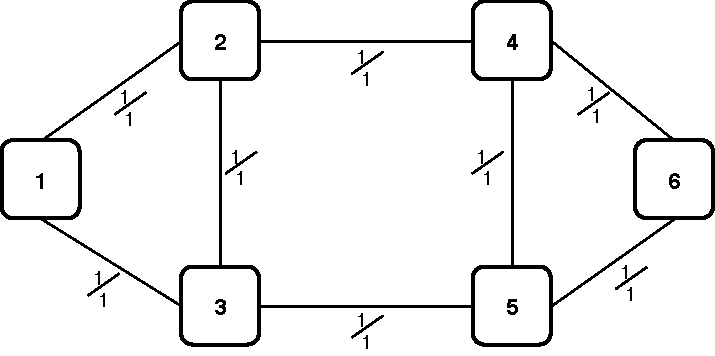
\includegraphics[width=12cm]{sdf/ilp/translucent_protection/figures/physical_topology}
\caption{Translucent with 1+1 protection in high scenario: Physical topology after dimensioning.}
\label{physical3_protectionhigh}
\end{figure}

\begin{figure}[h!]
\centering
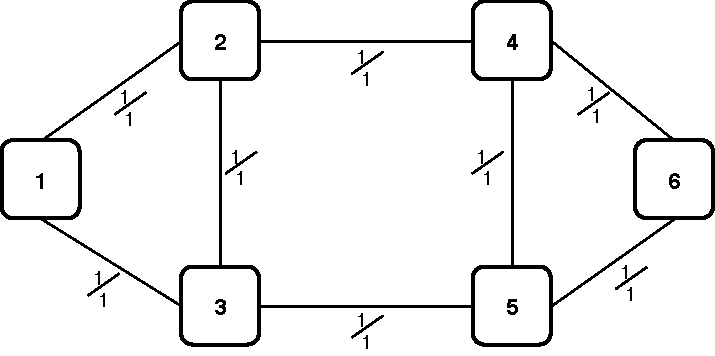
\includegraphics[width=12cm]{sdf/ilp/translucent_protection/figures/physical_topology}
\caption{Translucent with 1+1 protection in high scenario: Optical topology after dimensioning.}
\label{optical3_protectionhigh}
\end{figure}

In table \ref{link_transluc_protec_ref_high} we can see the number of optical channels calculated using \ref{Capex_Link} and \ref{ILPOpaque_CAPEX} and the number of amplifiers for each link calculated using \ref{Capex_amplifiers}.\\
In table \ref{node_transluc_protec_ref_high} we can see the resulting nodal degree at the physical layer, the number of line ports and add ports using \ref{OXC_poxc_transluc} the number of long-reach transponders using \ref{EXC_pexc2_transluc} and the number of tributary ports using \ref{EXC_pexc1_transluc}.\\
\newpage
\begin{table}[h!]
\centering
\begin{tabular}{|| c | c | c ||}
 \hline
 \multicolumn{3}{|| c ||}{Information regarding links} \\
 \hline
 \hline
 Bidirectional Link & Optical Channels & Amplifiers\\
 \hline
 Node 1 <-> Node 2 & 4 & 4 \\
 Node 1 <-> Node 3 & 4 & 6 \\
 Node 2 <-> Node 3 & 2 & 0 \\
 Node 2 <-> Node 4 & 14 & 6 \\
 Node 3 <-> Node 5 & 10 & 8 \\
 Node 4 <-> Node 5 & 8 & 1 \\
 Node 4 <-> Node 6 & 22 & 7 \\
 Node 5 <-> Node 6 & 18 & 3 \\
 \hline
\end{tabular}
\caption{Table with information regarding links for translucent mode with 1+1 protection in high scenario.}
\label{link_transluc_protec_ref_high}
\end{table}

\begin{table}[h!]
\centering
\begin{tabular}{|| c | c | c | c | c | c ||}
 \hline
 \multicolumn{6}{|| c ||}{Information regarding nodes} \\
 \hline
 \hline
 \multicolumn{2}{|| c |}{ } & \multicolumn{2}{ c |}{Electrical part} & \multicolumn{2}{ c ||}{Optical part} \\
 \hline
 Node & Resulting Nodal Degree & Tributary Ports & LR Transponders & Add Ports & Line Ports\\
 \hline
 1 & 2 & 290 & 8 & 8 & 8 \\
 2 & 3 & 230 & 20 & 20 & 20 \\
 3 & 3 & 180 & 16 & 16 & 16 \\
 4 & 3 & 200 & 24 & 24 & 44 \\
 5 & 3 & 240 & 24 & 24 & 36 \\
 6 & 2 & 220 & 40 & 40 & 40 \\
\hline
\end{tabular}
\caption{Table with information regarding nodes for translucent mode with 1+1 protection in high scenario.}
\label{node_transluc_protec_ref_high}
\end{table}

Through the information obtained previously on the nodes we can now create tables with detailed information about each node.

\begin{table}[h!]
\centering
\begin{tabular}{|| c | c | c ||}
 \hline
 \multicolumn{3}{|| c ||}{Detailed description of Node 1} \\
 \hline
 \hline
 Electrical part & Number of total demands & Bit rate \\
 \hline
\multirow{3}{*}{290 tributary ports} & 130 & ODU0 \\
 & 130 & ODU1 \\
 & 30 & ODU2 \\
 \hline
  & Node<--Optical Channels-->Node & Bit rate \\
 \hline
\multirow{2}{*}{8 LR Transponders} & 1  <---- 4 ---->  2 & \multirow{2}{*}{100 Gbits/s} \\
  & 1  <---- 4 ---->  3 & \\
 \hline
 \hline
 Optical part & Node<--Optical Channels-->Node & Bit rate \\
 \hline
 \multirow{2}{*}{8 add ports} & 1  <---- 4 ---->  2 & \multirow{4}{*}{100 Gbits/s} \\
  & 1  <---- 4 ---->  3 & \\ \cline{1-2}
 \multirow{2}{*}{8 line ports} & 1  <---- 4 ---->  2 & \\
  & 1  <---- 4 ---->  3 & \\
\hline
\end{tabular}
\caption{Translucent with 1+1 protection in high scenario: Detailed description of node 1. The number of demands is distributed to the various destination nodes, this distribution can be observed in section \ref{high_traffic_scenario}.}
\end{table}
\newpage
\begin{table}[h!]
\centering
\begin{tabular}{|| c | c | c ||}
 \hline
 \multicolumn{3}{|| c ||}{Detailed description of Node 2} \\
 \hline
 \hline
 Electrical part & Number of total demands & Bit rate \\ \hline
\multirow{5}{*}{230 tributary ports} & 110 & ODU0 \\
 & 70 & ODU1 \\
 & 20 & ODU2 \\
 & 20 & ODU3 \\
 & 10 & ODU4 \\
 \hline
  & Node<--Optical Channels-->Node & Bit rate \\
  \hline
\multirow{4}{*}{20 LR Transponders} & 2  <---- 4 ---->  1 & \multirow{4}{*}{100 Gbits/s} \\
  & 2  <---- 2 ---->  3 & \\
  & 2  <---- 4 ---->  4 & \\
  & 2  <---- 10 ---->  6 & \\
 \hline
 \hline
 Optical part & Node<--Optical Channels-->Node & Bit rate \\
 \hline
 \multirow{4}{*}{20 add ports} & 2  <---- 4 ---->  1 & \multirow{8}{*}{100 Gbits/s} \\
  & 2  <---- 2 ---->  3 & \\
  & 2  <---- 4 ---->  4 & \\
  & 2  <---- 10 ---->  6 & \\ \cline{1-2}
 \multirow{4}{*}{20 line ports} & 2  <---- 4 ---->  1 & \\
  & 2  <---- 2 ---->  3 & \\
  & 2  <---- 4 ---->  4 & \\
  & 2  <---- 10 ---->  6 & \\
\hline
\end{tabular}
\caption{Translucent with 1+1 protection in high scenario: Detailed description of node 2. The number of demands is distributed to the various destination nodes, this distribution can be observed in section \ref{high_traffic_scenario}.}
\end{table}

\begin{table}[h!]
\centering
\begin{tabular}{|| c | c | c ||}
 \hline
 \multicolumn{3}{|| c ||}{Detailed description of Node 4} \\
 \hline
 \hline
 Electrical part & Number of total demands & Bit rate \\ \hline
\multirow{3}{*}{200 tributary ports} & 70 & ODU0 \\
 & 100 & ODU1 \\
 & 30 & ODU2 \\
 \hline
  & Node<--Optical Channels-->Node & Bit rate \\ \hline
 \multirow{3}{*}{24 LR Transponders} & 4  <---- 4 ---->  2 & \multirow{3}{*}{100 Gbits/s} \\
  & 4  <---- 8 ---->  5 & \\
  & 4  <---- 12 ---->  6 & \\
 \hline
 \hline
 Optical part & Node<--Optical Channels-->Node & Bit rate \\
 \hline
 \multirow{3}{*}{24 add ports} & 4  <---- 4 ---->  2 & \multirow{7}{*}{100 Gbits/s} \\
  & 4  <---- 8 ---->  5 & \\
  & 4  <---- 12 ---->  6 & \\ \cline{1-2}
 \multirow{4}{*}{44 line ports} & 4  <---- 4 ---->  2 & \\
  & 4  <---- 8 ---->  5 & \\
  & 4  <---- 12 ---->  6 & \\
  & 2  <---- 10 ---->  6 & \\
\hline
\end{tabular}
\caption{Translucent with 1+1 protection in high scenario: Detailed description of node 4. The number of demands is distributed to the various destination nodes, this distribution can be observed in section \ref{high_traffic_scenario}.}
\end{table}

\newpage
\begin{table}[h!]
\centering
\begin{tabular}{|| c | c | c ||}
 \hline
 \multicolumn{3}{|| c ||}{Detailed description of Node 3} \\
 \hline
 \hline
 Electrical part & Number of total demands & Bit rate \\
 \hline
 \multirow{4}{*}{180 tributary ports} & 70 & ODU0 \\
 & 60 & ODU1\\
 & 30 & ODU2\\
 & 20 & ODU3\\
 \hline
  & Node<--Optical Channels-->Node & Bit rate \\ \hline
 \multirow{4}{*}{16 LR Transponders} & 3  <---- 4 ---->  1 & \multirow{4}{*}{100 Gbits/s} \\
  & 3  <---- 2 ---->  2 & \\
  & 3  <---- 4 ---->  5 & \\
  & 3  <---- 6 ---->  6 & \\
 \hline
 \hline
 Optical part & Node<--Optical Channels-->Node & Bit rate \\
 \hline
 \multirow{4}{*}{16 add ports} & 3  <---- 4 ---->  1 & \multirow{8}{*}{100 Gbits/s} \\
  & 3  <---- 2 ---->  2 & \\
  & 3  <---- 4 ---->  5 & \\
  & 3  <---- 6 ---->  6 & \\ \cline{1-2}
 \multirow{4}{*}{16 line ports} & 3  <---- 4 ---->  1 & \\
  & 3  <---- 2 ---->  2 & \\
  & 3  <---- 4 ---->  5 & \\
  & 3  <---- 6 ---->  6 & \\
\hline
\end{tabular}
\caption{Translucent with 1+1 protection in high scenario: Detailed description of node 3. The number of demands is distributed to the various destination nodes, this distribution can be observed in section \ref{high_traffic_scenario}.}
\end{table}

\begin{table}[h!]
\centering
\begin{tabular}{|| c | c | c ||}
 \hline
 \multicolumn{3}{|| c ||}{Detailed description of Node 6} \\
 \hline
 \hline
 Electrical part & Number of total demands & Bit rate \\ \hline
\multirow{5}{*}{220 tributary ports} & 80 & ODU0 \\
 & 100 & ODU1 \\
 & 10 & ODU2 \\
 & 10 & ODU3 \\
 & 20 & ODU4 \\
 \hline
  & Node<--Optical Channels-->Node & Bit rate \\ \hline
 \multirow{3}{*}{20 LR Transponders} & 6  <---- 4 ---->  2 & \multirow{3}{*}{100 Gbits/s} \\
  & 6  <---- 2 ---->  4 & \\
  & 6  <---- 14 ---->  5 & \\
 \hline
 Optical part & Node<--Optical Channels-->Node & Bit rate \\
 \hline
 \multirow{3}{*}{20 add ports} & 6  <---- 4 ---->  2 & \multirow{6}{*}{100 Gbits/s} \\
  & 6  <---- 2 ---->  4 & \\
  & 6  <---- 14 ---->  5 & \\ \cline{1-2}
 \multirow{3}{*}{20 line ports} & 6  <---- 4 ---->  2 & \\
  & 6  <---- 2 ---->  4 & \\
  & 6  <---- 14 ---->  5 & \\
\hline
\end{tabular}
\caption{Translucent with 1+1 protection in high scenario: Detailed description of node 6. The number of demands is distributed to the various destination nodes, can be observed in section \ref{high_traffic_scenario}.}
\end{table}

\newpage
\begin{table}[h!]
\centering
\begin{tabular}{|| c | c | c ||}
 \hline
 \multicolumn{3}{|| c ||}{Detailed description of Node 5} \\
 \hline
 \hline
 Electrical part & Number of total demands & Bit rate \\ \hline
\multirow{5}{*}{240 tributary ports} & 140 & ODU0 \\
 & 40 & ODU1 \\
 & 40 & ODU2 \\
 & 10 & ODU3 \\
 & 10 & ODU4 \\
 \hline
  & Node<--Optical Channels-->Node & Bit rate \\ \hline
 \multirow{3}{*}{24 LR Transponders} & 5  <---- 4 ---->  3 & \multirow{3}{*}{100 Gbits/s} \\
  & 5  <---- 8 ---->  4 & \\
  & 5  <---- 12 ---->  6 & \\
 \hline
 \hline
 Optical part & Node<--Optical Channels-->Node & Bit rate \\
 \hline
 \multirow{3}{*}{24 add ports} & 5  <---- 4 ---->  3 & \multirow{7}{*}{100 Gbits/s} \\
  & 5  <---- 8 ---->  4 & \\
  & 5  <---- 12 ---->  6 & \\ \cline{1-2}
 \multirow{4}{*}{36 line ports} & 5  <---- 4 ---->  3 & \\
  & 5  <---- 8 ---->  4 & \\
  & 5  <---- 12 ---->  6 & \\
  & 3  <---- 6 ---->  6 & \\
\hline
\end{tabular}
\caption{Translucent with 1+1 protection in high scenario: Detailed description of node 5. The number of demands is distributed to the various destination nodes, this distribution can be observed in section \ref{high_traffic_scenario}.}
\end{table}

Now through table \ref{scripttransluc_protec_ref_high} we can see the CAPEX result for this model. This value is obtained using equation \ref{Capex} and all of the constraints mentioned above.

\begin{table}[h!]
\centering
\begin{tabular}{|| c | c | c | c | c | c | c ||}
 \hline
 \multicolumn{7}{|| c ||}{CAPEX of the Network} \\
 \hline
 \hline
 \multicolumn{3}{|| c |}{ } & Quantity & Unit Price & Cost & Total \\
 \hline
 \multirow{3}{*}{Link Cost} & \multicolumn{2}{ c |}{OLTs} & 16 & 15 000 \euro & 240 000 \euro & \multirow{3}{*}{82 520 000 \euro} \\ \cline{2-6}
 & \multicolumn{2}{ c |}{100 Gbits/s Transceivers} & 164 & 5 000 \euro/Gbit/s & 82 000 000 \euro & \\ \cline{2-6}
 & \multicolumn{2}{ c |}{Amplifiers} & 70 & 4 000 \euro & 280 000 \euro & \\
 \hline
 \multirow{10}{*}{Node Cost} & \multirow{7}{*}{Electrical} & EXCs & 6 & 10 000 \euro & 60 000 \euro & \multirow{10}{*}{14 145 900 \euro} \\ \cline{3-6}
 & & ODU0 Ports & 600 & 10 \euro/port & 6 000 \euro & \\ \cline{3-6}
 & & ODU1 Ports & 500 & 15 \euro/port & 7 500 \euro & \\ \cline{3-6}
 & & ODU2 Ports & 160 & 30 \euro/port & 4 800 \euro & \\ \cline{3-6}
 & & ODU3 Ports & 60 & 60 \euro/port & 3 600 \euro & \\ \cline{3-6}
 & & ODU4 Ports & 40 & 100 \euro/port & 4 000 \euro & \\ \cline{3-6}
 & &Transponders& 132 & 100 000 \euro/port & 13 200 000 \euro & \\ \cline{2-6}
 & \multirow{3}{*}{Optical} & OXCs & 6 & 20 000 \euro & 120 000 \euro & \\ \cline{3-6}
 & & Line Ports & 164 & 2 500 \euro/port & 410 000 \euro & \\ \cline{3-6}
 & & Add Ports & 132 & 2 500 \euro/port & 330 000 \euro & \\
 \hline
 \multicolumn{6}{|| c |}{Total Network Cost} & 96 665 900 \euro \\
\hline
\end{tabular}
\caption{Translucent with 1+1 protection in high scenario: Detailed description of CAPEX for this scenario.}
\label{scripttransluc_protec_ref_high}
\end{table}

In next page, let's focus on the routing information. These paths are bidirectional so the path from one node to another is the same path in the opposite direction.

\newpage
\begin{table}[h]
\centering
\begin{tabular}{||c|c|c|c|c||}
 \hline
 \multicolumn{5}{|| c ||}{Routing} \\
 \hline
 \hline
 o & d & Type & Links & Demands \\
 \hline
 \multirow{2}{*}{1}&\multirow{2}{*}{2}&W&\{(1,3),(3,5),(5,6),(6,4),(4,2)\}&50 ODU0, 20 ODU1, 10 ODU2\\
  & &P& \{(1,2)\} &50 ODU0, 20 ODU1, 10 ODU2 \\ \hline
 \multirow{2}{*}{1}&\multirow{2}{*}{3}&W& \{(1,2),(2,3)\} & 10 ODU0, 40 ODU1, 10 ODU2\\
  & &P& \{(1,3)\} & 10 ODU0, 40 ODU1, 10 ODU2 \\ \hline
 \multirow{2}{*}{1} & \multirow{2}{*}{4}&W&\{(1,3),(3,5),(5,6),(6,4)\}&30 ODU0, 20 ODU1, 10 ODU2\\
  & &P& \{(1,2),(2,4)\} & 30 ODU0, 20 ODU1, 10 ODU2 \\ \hline
 \multirow{2}{*}{1} & \multirow{2}{*}{5}&W&\{(1,2),(2,4),(4,5)\}& 10 ODU0\\
  & &P& \{(1,3),(3,5)\} & 10 ODU0 \\ \hline
 \multirow{2}{*}{1} & \multirow{2}{*}{6}&W& \{(1,3),(3,5),(5,6)\} & 30 ODU0, 50 ODU1 \\
  & &P& \{(1,2),(2,4),(4,6)\} & 30 ODU0, 50 ODU1 \\ \hline
 \multirow{4}{*}{2} & \multirow{4}{*}{3}&W& \{(2,1),(1,3)\} & 5 ODU3 \\
  & &W& \{(2,4),(4,6),(6,5),(5,3)\} & 5 ODU3 \\
  & &P& \{(2,3)\} & 5 ODU3 \\
  & &P& \{(2,1),(1,3)\} & 5 ODU3 \\ \hline
 \multirow{2}{*}{2} & \multirow{2}{*}{4}&W&\{(2,4),(4,6),(6,4)\}&10 ODU0, 30 ODU1 \\
  & &P& \{(2,4)\} & 10 ODU0, 30 ODU1 \\ \hline
 \multirow{4}{*}{2} & \multirow{4}{*}{5}&W&\{(2,4),(4,5)\} & 50 ODU0, 10 ODU1 \\
  & &W& \{(2,1),(1,3),(3,5)\} & 1 ODU2 \\
  & &P& \{(2,3),(3,5)\} & 50 ODU0, 10 ODU1 \\
  & &P& \{(2,4),(4,5)\} & 1 ODU2 \\ \hline
 \multirow{4}{*}{2} & \multirow{4}{*}{6}&W&\{(2,3),(3,5),(5,6)\}& 10 ODU1, 2 ODU4 \\
  & &W& \{(2,4),(4,6)\} & 10 0DU3, 4 ODU4 \\
  & &W& \{(2,1),(1,3),(3,5),(5,6)\} & 4 ODU4 \\
  & &P& \{(2,4),(4,6)\} & 10 ODU1, 10 ODU3, 10 ODU4 \\ \hline
 \multirow{2}{*}{3} & \multirow{2}{*}{4}&W& \{(3,5),(5,6),(6,4)\} & 10 ODU0, 10 ODU1, 10 ODU2 \\
  & &P& \{(3,2),(2,4)\} & 10 ODU0, 10 ODU1, 10 ODU2 \\ \hline
 \multirow{3}{*}{3}&\multirow{3}{*}{5}&W&\{(3,2),(2,4),(4,5)\}&40 ODU0, 10 ODU1 \\
  & &W& \{(3,5),(5,6),(6,4),(4,5)\}& 10 ODU2, 10 ODU3\\
  & &P& \{(3,5)\} & 40 ODU0, 10 ODU1, 10 ODU2, 10 ODU3 \\ \hline
 \multirow{2}{*}{3} & \multirow{2}{*}{6}&W& \{(3,2),(2,4),(4,6)\} & 10 ODU0 \\
  & &P& \{(3,6)\} & 10 ODU0 \\ \hline
 \multirow{3}{*}{4} & \multirow{3}{*}{5}&W& \{(4,2),(2,3),(3,5)\} & 10 ODU0 \\
  & &W& \{(4,6),(6,5),(5,3),(3,5)\} & 10 ODU1, 10 ODU2 \\
  & &P& \{(4,5)\} & 10 ODU0, 10 ODU1, 10 ODU2 \\ \hline
 \multirow{2}{*}{4} & \multirow{2}{*}{6}&W& \{(4,2),(2,4),(4,6)\} & 10 ODU0, 30 ODU1\\
  & &P& \{(4,6)\} & 10 ODU0, 30 ODU1\\ \hline
 \multirow{3}{*}{5} & \multirow{3}{*}{6}&W&\{(5,3),(3,5),(5,6)\}& 30 ODU0, 10 ODU1, 10 ODU2, 2 ODU4 \\
  & &W& \{(5,4),(4,6)\} & 8 ODU4 \\
  & &P& \{(5,6)\}& 30 ODU0, 10 ODU1, 10 ODU2, 10 ODU4 \\ \hline
\end{tabular}
\caption{Translucent with 1+1 protection in high scenario: Description of demands routing. The type W means that it is working path and type P protection path.}
\label{path_transluc_protec_ref_high}
\end{table}
\newpage
